\documentclass[11pt]{beamer}

\usepackage{cedilleverbatim}
\usepackage{times}
\usepackage[absolute,overlay]{textpos}
\usepackage{stmaryrd}
\usepackage{MnSymbol}
\usepackage[normalem]{ulem} %for \sout

\usepackage{tikz}
\usepackage{graphicx}
%\usepackage{epstopdf}
\usepackage{color}
%\usepackage{tabularx}
\usepackage{pgflibraryarrows}
\usepackage{pgflibraryshapes}
\usepackage{pgfbaseimage}
\usepackage{listings}

\usetikzlibrary{decorations.text}

%\documentclass{beamer}
%\usepackage{beamerthemesplit}
%\usepackage{mathptmx}
%\usepackage{helvet}

%\usepackage{amsmath}
\usepackage{latexsym}
%\usepackage{amssymb}
\usepackage{proof}
\usepackage{verbatim} 
\usepackage{url}

\definecolor{navy}{RGB}{0,0,128}
\definecolor{dorange}{RGB}{255,100,0}
\definecolor{dgreen}{RGB}{0,75,0}
\definecolor{dbrown}{RGB}{125,30,0}
\definecolor{lbrown}{RGB}{245,150,120}
\definecolor{ored}{RGB}{255,150,70}
\definecolor{oredd}{RGB}{255,69,0}
\definecolor{lightred}{RGB}{255,70,70}
\definecolor{vlred}{RGB}{255,170,170}
\definecolor{cream}{RGB}{255,253,208}
\definecolor{lthistle}{RGB}{185,175,185}

\newcommand{\semeq}[1]{\langle\hspace{-.08cm}|#1|\hspace{-0.08cm}\rangle}
\newcommand{\rep}[1]{\ulcorner #1 \urcorner}
\newcommand{\tlift}[2]{{\uparrow}_{#1}\,(#2)}
\newcommand{\dstar}[0]{\smallstar}
\newcommand{\utp}[0]{\mathcal{U}}
\newcommand{\elcap}[0]{\cap}
\newcommand{\nutt}[4]{\nu\, #1\! :\! #2 \, |\, #3.\, #4}
\newcommand{\interp}[1]{\llbracket #1 \rrbracket} 
\newcommand{\abs}[4]{{#1}\, #2\! : \! #3.\, #4}

% unicode
\usepackage[utf8]{inputenc}
\DeclareUnicodeCharacter{2605}{\ensuremath{\star}}
\DeclareUnicodeCharacter{2081}{\ensuremath{_1}}
\DeclareUnicodeCharacter{2082}{\ensuremath{_2}}
\DeclareUnicodeCharacter{2228}{\ensuremath{\vee}}
\DeclareUnicodeCharacter{27E6}{\ensuremath{\llbracket}}
\DeclareUnicodeCharacter{27E7}{\ensuremath{\rrbracket}}
\DeclareUnicodeCharacter{228E}{\ensuremath{\uplus}}
\DeclareUnicodeCharacter{2113}{\ensuremath{\ell}}
\DeclareUnicodeCharacter{2294}{\ensuremath{\sqcup}}
\DeclareUnicodeCharacter{2192}{\ensuremath{\to}}
\DeclareUnicodeCharacter{2200}{\ensuremath{\forall}}
\DeclareUnicodeCharacter{22CE}{\ensuremath{\curlyvee}}
\DeclareUnicodeCharacter{2115}{\ensuremath{\mathbb{N}}}
\DeclareUnicodeCharacter{2238}{\ensuremath{\dotdiv}}
\DeclareUnicodeCharacter{2261}{\ensuremath{\equiv}}
\DeclareUnicodeCharacter{3BB}{\ensuremath{\lambda}}
\DeclareUnicodeCharacter{1D539}{\ensuremath{\mathbb{B}}}
\DeclareUnicodeCharacter{1D543}{\ensuremath{\mathbb{L}}}
\DeclareUnicodeCharacter{1D54A}{\ensuremath{\mathbb{S}}}
\DeclareUnicodeCharacter{1D54B}{\ensuremath{\mathbb{T}}}
\DeclareUnicodeCharacter{1D54D}{\ensuremath{\mathbb{V}}}
\DeclareUnicodeCharacter{D7}{\ensuremath{\times}}
\DeclareUnicodeCharacter{25C2}{\ensuremath{:}}

\newcommand{\myb}[0]{\ensuremath{\textcolor{blue}{\triangleright}}}

\newcommand{\fore}[0]{\ensuremath{F_\omega^{\textit{rec}}}}


\mode<presentation>
{
  %\usetheme{Warsaw}
  % or ...

%\usetheme{IowaCity}
\usetheme{Boston}
%\usetheme{Savannah}

%  \setbeamercovered{transparent}
  % or whatever (possibly just delete it)
}

\usepackage[english]{babel}
% or whatever

\usepackage{times}
\usepackage[T1]{fontenc}
% Or whatever. Note that the encoding and the font should match. If T1
% does not look nice, try deleting the line with the fontenc.



\date{\ }

\begin{document}


\setbeamercolor{normal text}{bg=white,fg=black}

\begin{frame}

\begin{center}
{\huge
  Introduction to Programming and

\vspace{.1cm}

  Proving in Cedille }

\vspace{.75cm}

\includegraphics[width=3cm]{logo}

%\includegraphics[width=5cm]{oldcap}

\vspace{.6cm}

Chris Jenkins, Colin McDonald, Aaron Stump

{\small
Computer Science 

The University of Iowa

Iowa City, Iowa}

\end{center}
\end{frame}

\newcommand{\grun}[1]{\textcolor{dgreen}{\underline{#1}}}

\newcommand{\qlogo}[1]{\raisebox{-.25\height}{\includegraphics[width=#1]{logo}}?}

\newenvironment{planslide}[1]{%
\begin{frame}
\frametitle{Plan for the tutorial}

\large 

\begin{tabular}{l c l }

\qlogo{.7cm} &\ & \textcolor{#1}{Motivation and background for Cedille} \\ \\


$\vdash \textit{\textcolor{red}{C}e\textcolor{red}{D}il\textcolor{red}{LE}}$ &\ & \textcolor{#1}{Syntax and semantics}\\ \\

\texttt{cedille} &\ & \textcolor{#1}{Tooling: emacs frontend $\leftrightarrow$ backend} \\ \\

$\leadsto\ \texttt{cedille}_{\texttt{core}}$ & \ & \textcolor{#1}{Elaboration to Cedille Core} \\ \\

\texttt{c d ll} &\ & \textcolor{#1}{Spine-local type inference} \\ \\ 

%\begin{tikzpicture}[
%  decoration={
%    reverse path,
%    text effects along path,
%    text={cedille cedille cedille cedille cedille cedille cedille cedille cedille cedille cedille cedille cedille cedille
%      cedille cedille cedille cedille cedille cedille cedille cedille cedille.},
%    text effects/.cd,
%      text along path,
%      character count=\i, character total=\n,
%      characters={scale=1-\i/\n}
%    }
%]
%\draw [decorate] (0,0) 
%    \foreach \i [evaluate={\r=(\i/2400)^2;}] in {0,7,...,2380}{ -- (\i:\r)}; 
%\end{tikzpicture}

\raisebox{-.8\height}{\includegraphics[width=2cm]{cedillespiral}} &\ & 

\textcolor{#1}{Future directions}


\end{tabular}

\end{frame}
}

\planslide{white}
\planslide{red}

\begin{frame}
\begin{center}
  \Huge
  \qlogo{1.8
    cm}

  \vspace{1cm}

{\Large
  \textcolor{red}{Motivation and background for Cedille}
}
  \end{center}

\end{frame}

\begin{frame}
\frametitle{A little history}

\pause
\begin{center}
\includegraphics[width=4in]{bonnevillesign}
\end{center}

\end{frame}

\setlength{\TPHorizModule}{.1cm}
\setlength{\TPVertModule}{.1cm}
\setbeamercolor{mycolor}{fg=black,bg=white}

\newcommand{\carbox}[4]{%
\begin{tikzpicture}
    \node at (0,0) {#1};
    \node at (-2.68,-4.2) {\small \emph{#4}};
    \pause
    \node at #2 {#3};

\end{tikzpicture}
}

\begin{frame}
  \frametitle{System F (Girard, Reynolds, early 1970s)}

  \carbox{\includegraphics[width=4in]{bonneville1}}{(0,2.5)}{\begin{minipage}{7cm}
  \begin{beamercolorbox}{mycolor}
        \begin{itemize}
        \item[$\myb$] $\forall\ X : \star.\ T$
        \item[$\myb$] Raw power (\textcolor{blue}{impredicativity!})
        \item[$\myb$] A little crude (\textcolor{red}{no Curry-Howard})
          \vspace{.25cm}
          \end{itemize}
                    \end{beamercolorbox}\end{minipage}}{1969 Mercury Cyclone Spoiler II}

    \end{frame}

\begin{frame}
  \frametitle{Calculus of Constructions (Coquand, Huet 1988)}

  \carbox{\includegraphics[width=4in]{camaro}}{(0,2.4)}{\begin{minipage}{9cm}
      \begin{beamercolorbox}{mycolor}
        \begin{itemize}
        \item[$\myb$] Add dependent types: $\Pi\ x : T.\ T'$
        \item[$\myb$] Imported from Automath/Martin-L\"of type theory
        \item[$\myb$] \textcolor{blue}{Curry-Howard!}
        \item[$\myb$] \textcolor{red}{No induction.} [Geuvers 2001]
        \end{itemize}
        \end{beamercolorbox}\end{minipage}}{1988 Chevrolet Camaro}

\end{frame}

\begin{frame}
  \frametitle{Calculus of Inductive Constructions (Werner 1994)}

  \carbox{\includegraphics[width=4in]{streamliner}}{(0,1.8)}{\begin{minipage}{9cm}
      \begin{beamercolorbox}{mycolor}
        \begin{itemize}
        \item[$\myb$] Add primitive inductive types
        \item[$\myb$] Finally ready for constructive mathematics!
        \item[$\myb$] Basis for Coq
        \end{itemize}
        \end{beamercolorbox}\end{minipage}}{1992 Hoffman-Markley Streamliner}
\end{frame}

\begin{frame}
  \frametitle{But Coq $\neq$ CIC}

  \begin{itemize}
  \item[$\myb$] Coinductive types
  \item[$\myb$] Universe hierarchy (Extended CC, Luo 1990)
  \item[$\myb$] Proof-irrelevant universe \texttt{Prop}
  \item[$\myb$] \emph{And we might want more:}
    \begin{itemize}
    \item definitional proof irrelevance
    \item inductive-inductive types
    \item inductive-recursive types
      \end{itemize}
  \end{itemize}

\vspace{.5cm}

  Similarly, Agda $\neq$ MLTT.

\vspace{.5cm}

\end{frame}

\begin{frame}
  \frametitle{Issues and limitations, Coq and Agda}

  \begin{itemize}
  \item[$\myb$] No formal semantics/correctness proof
    \begin{itemize}
    \item Despite a lot of interest: TT in TT
      \end{itemize}

\vspace{.1cm}

  \item[$\myb$] (\textcolor{blue}{Hence!}) bugs and surprises
    \begin{itemize}
    \item[$\myb$] incompatibilities with various axioms
    \item[$\myb$] actual contradictions!
    \item[$\myb$] type soundness broken in Coq
    \end{itemize}

\vspace{.1cm}

  \item[$\myb$] Commitment to a set of datatypes
    \begin{itemize}
      \item[$\myb$] theory of datatypes not finished...
      \item[$\myb$] e.g., higher-order abstract syntax prohibited
    \end{itemize}
  \end{itemize}
\end{frame}

\newcommand{\monsterf}[1]{\begin{frame}
  \frametitle{Have we created a monster?}

  \includegraphics[width=4.5in]{#1}

  {\small \emph{Schaufelradbagger 258}}

\end{frame}
}

\monsterf{bagger258a}
\monsterf{bagger258b}

\begin{frame}
  \frametitle{\emph{If I could turn back time...}}

  \begin{columns}
\hspace{.5cm}    \column{2.8in}

  Good-bye to:

  \begin{itemize}
  \item[$\myb$] primitive datatypes
  \item[$\myb$] (also universe hierarchy, my bias)
  \end{itemize}

\vspace{.2cm}

  For this, hello to

  \begin{itemize}
  \item[$\myb$] lambda-encodings of data
  \end{itemize}

  \column{2.6in}
  \onslide<2>{\includegraphics[width=1.8in]{cher}}
  \end{columns}

  \onslide<3>{\ }
  \end{frame}

\begin{frame}
  \frametitle{\colorbox{black}{\textcolor{white}{Wanted}}: \textcolor{red}{a new type theory} }

  where

  \begin{itemize}
  \item[$\myb$] inductive datatypes are \underline{derived} (lambda-encoded)
  \item[$\myb$] impredicativity is central
  \item[$\myb$] core theory is small and verifiable
  \end{itemize}

\vspace{.15cm}

  Tooling goals:

  \begin{itemize}
  \item[$\myb$] see all typing/inference information 
  \item[$\myb$] predictable inference
  \item[$\myb$] elaborate to core with independent checker
  \end{itemize}

\end{frame}

\begin{frame}
  \frametitle{This is Cedille}

  \end{frame}

\begin{frame}
  \frametitle{Architecture of Cedille}

\hspace{1cm}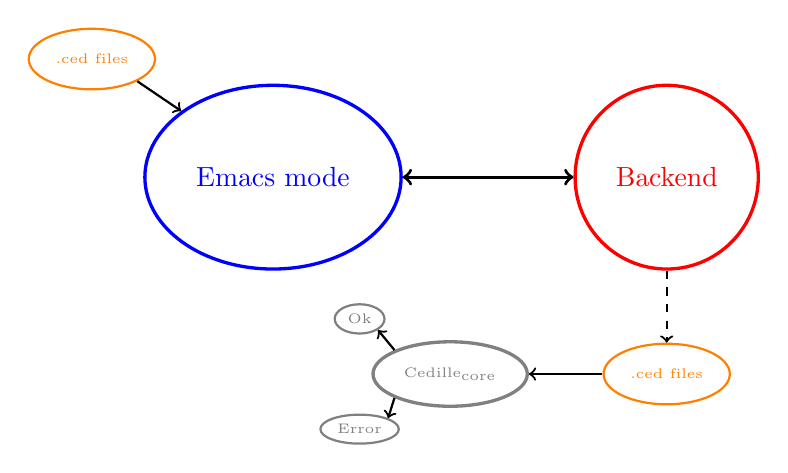
\begin{tikzpicture}

\path (1,2.5) node[very thick,blue,ellipse,draw,inner xsep=5pt,inner ysep=20pt](emacsmode){Emacs mode} ;
\path (6,2.5) node[very thick,red,ellipse,draw,inner xsep=5pt,inner ysep=20pt](backend){Backend} ;

\path (-1.3,4) node[thick,orange,ellipse,draw,inner xsep=3pt,inner ysep=6pt](cedfilesa){{\tiny .ced files}} ;

\draw[<->,very thick,black] (emacsmode.east) -- (backend.west);
\draw[->,thick,black] (cedfilesa.south east) -- (emacsmode.north west);

\pause

\path (6,0) node[thick,orange,ellipse,draw,inner xsep=3pt,inner ysep=6pt](cedfilesb){{\tiny .ced files}} ;

\path (3.25,0) node[very thick,gray,ellipse,draw,inner xsep=3pt,inner ysep=6pt](cedillecore){{\tiny Cedille\textsubscript{core}}} ;
\path (2.1,0.7) node[thick,gray,ellipse,draw,inner xsep=2pt,inner ysep=2pt](cedillecoreok){{\tiny Ok}} ;
\path (2.1,-0.7) node[thick,gray,ellipse,draw,inner xsep=2pt,inner ysep=2pt](cedillecoreerr){{\tiny Error}} ;

\draw[->,thick,black,dashed] (backend.south) -- (cedfilesb.north);
\draw[->,thick,black] (cedfilesb.west) -- (cedillecore.east);
\draw[->,thick,black] (cedillecore.north west) -- (cedillecoreok.south east);
\draw[->,thick,black] (cedillecore.south west) -- (cedillecoreerr.north east);

\end{tikzpicture}

\end{frame}

\begin{frame}
\frametitle{Emacs mode (\emph{to be revised})}

\begin{itemize}
\item Cedille has an emacs mode for editing Cedille files
\item Based on a generic structured-editing mode by Carl Olson

\vspace{.25cm}

\hspace{1cm}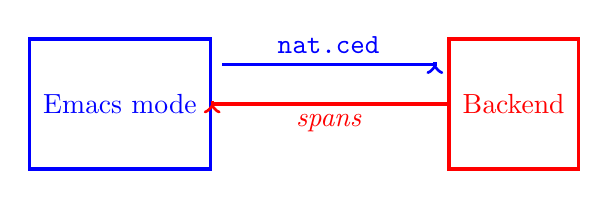
\begin{tikzpicture}

\path (1,0) node[very thick,blue,rectangle,draw,inner xsep=5pt,inner ysep=20pt](l){Emacs mode} ;
\path (6,0) node[very thick,red,rectangle,draw,inner xsep=5pt,inner ysep=20pt](r){Backend} ;

\draw[->,very thick,blue] (2.3,0.5) -| node[pos=0.25,above] {\texttt{nat.ced}} (5.0,0.5);
\draw[->,very thick,red] (r.west) -| node[pos=0.25,below] {\textit{spans}} (l.east);

\end{tikzpicture}

\vspace{.1cm}

\item A span is $[\textit{label},\textit{start-pos},\textit{end-pos},\textit{attributes}]$

\item Spans communicated in JSON

\item Cedille sends \underline{all} type information, in span attributes

\item Monadic style for writing the backend (type checker)

\end{itemize}
\end{frame}

\end{document}
